\documentclass[]{article}
\usepackage{lmodern}
\usepackage{amssymb,amsmath}
\usepackage{ifxetex,ifluatex}
\usepackage{fixltx2e} % provides \textsubscript
\ifnum 0\ifxetex 1\fi\ifluatex 1\fi=0 % if pdftex
  \usepackage[T1]{fontenc}
  \usepackage[utf8]{inputenc}
\else % if luatex or xelatex
  \ifxetex
    \usepackage{mathspec}
  \else
    \usepackage{fontspec}
  \fi
  \defaultfontfeatures{Ligatures=TeX,Scale=MatchLowercase}
\fi
% use upquote if available, for straight quotes in verbatim environments
\IfFileExists{upquote.sty}{\usepackage{upquote}}{}
% use microtype if available
\IfFileExists{microtype.sty}{%
\usepackage[]{microtype}
\UseMicrotypeSet[protrusion]{basicmath} % disable protrusion for tt fonts
}{}
\PassOptionsToPackage{hyphens}{url} % url is loaded by hyperref
\usepackage[unicode=true]{hyperref}
\hypersetup{
            pdftitle={Paper\_Draft},
            pdfauthor={Kate Saunders},
            pdfborder={0 0 0},
            breaklinks=true}
\urlstyle{same}  % don't use monospace font for urls
\usepackage[margin=1in]{geometry}
\usepackage{graphicx,grffile}
\makeatletter
\def\maxwidth{\ifdim\Gin@nat@width>\linewidth\linewidth\else\Gin@nat@width\fi}
\def\maxheight{\ifdim\Gin@nat@height>\textheight\textheight\else\Gin@nat@height\fi}
\makeatother
% Scale images if necessary, so that they will not overflow the page
% margins by default, and it is still possible to overwrite the defaults
% using explicit options in \includegraphics[width, height, ...]{}
\setkeys{Gin}{width=\maxwidth,height=\maxheight,keepaspectratio}
\IfFileExists{parskip.sty}{%
\usepackage{parskip}
}{% else
\setlength{\parindent}{0pt}
\setlength{\parskip}{6pt plus 2pt minus 1pt}
}
\setlength{\emergencystretch}{3em}  % prevent overfull lines
\providecommand{\tightlist}{%
  \setlength{\itemsep}{0pt}\setlength{\parskip}{0pt}}
\setcounter{secnumdepth}{0}
% Redefines (sub)paragraphs to behave more like sections
\ifx\paragraph\undefined\else
\let\oldparagraph\paragraph
\renewcommand{\paragraph}[1]{\oldparagraph{#1}\mbox{}}
\fi
\ifx\subparagraph\undefined\else
\let\oldsubparagraph\subparagraph
\renewcommand{\subparagraph}[1]{\oldsubparagraph{#1}\mbox{}}
\fi

% set default figure placement to htbp
\makeatletter
\def\fps@figure{htbp}
\makeatother


\title{Paper\_Draft}
\author{Kate Saunders}
\date{12/06/2020}

\begin{document}
\maketitle

\section{Introduction}\label{introduction}

Individually both extreme rainfall and storm surge pose a flood risk. If
these events co-occur, they create a compound event ({\textbf{???}}) and
the risk may be magnified compared to if either event occurred
individually. To reliably assess the flood risk from rainfall and surge
events, the dependence relationship between these events must be
accurately modelled (Zheng et al. 2014, Zscheischler and Seneviratne
(2017)).

The same is true for weather forecasts. To ensure communties aren't
caught unprepared, the accuracy of the joint forecast of must be
considered. These joint forecasts are needed to provide advance
warnings, so that the flood impacts are mitigated and water can be
released in advance from devices, such as sluces or pumps.

Weather processes however, are highly chaotic and complex. Therefore
forecasts from numerical weather models (NWP) can only serve as our
best, most-informed guesses of what the future weather will be. Even at
the high resolutions, these models contain systematic errors due to
simplyfing assumptions in their equations and compuational capacity
limits the number of future possible forecasts, so the full predictive
distribution can not be simulated. Statistical post-processing is
therefore needed to improve upon the reliabilitiy and accuracy of the
forecasts by reducing systematic errors, such as bias or dispersion
errors (({\textbf{???}}), ({\textbf{???}})).

Provide a post-processing summary and fill the gap

For forecasting the co-occurrence of bivariate events, such as rainfall
and storm surge, it is important to understand the driving mechanism
behind these events. (Wahl et al. 2015) breaks the compound event
mechanism into three types:

\begin{itemize}
\tightlist
\item
  \textbf{Mechanism (1)} in estuarine regions, the joint occurrence of
  both may elevate water levels to a point where flooding is initiated
  or its impacts exacerbated.\\
\item
  \textbf{Mechanism (2)} occurs when a destructive storm surge already
  causes widespread flooding, such that any significant rainfall on top
  of this---even if it is not an extreme event on its own---increases
  the flood depth and/or extent of the inundated area.\\
\item
  \textbf{Mechanism (3)} occurs during a moderate storm surge which does
  not directly cause flooding, but is high enough to fully block or slow
  down gravity-fed storm water drainage, such that precipitation is more
  likely to cause flooding.
\end{itemize}

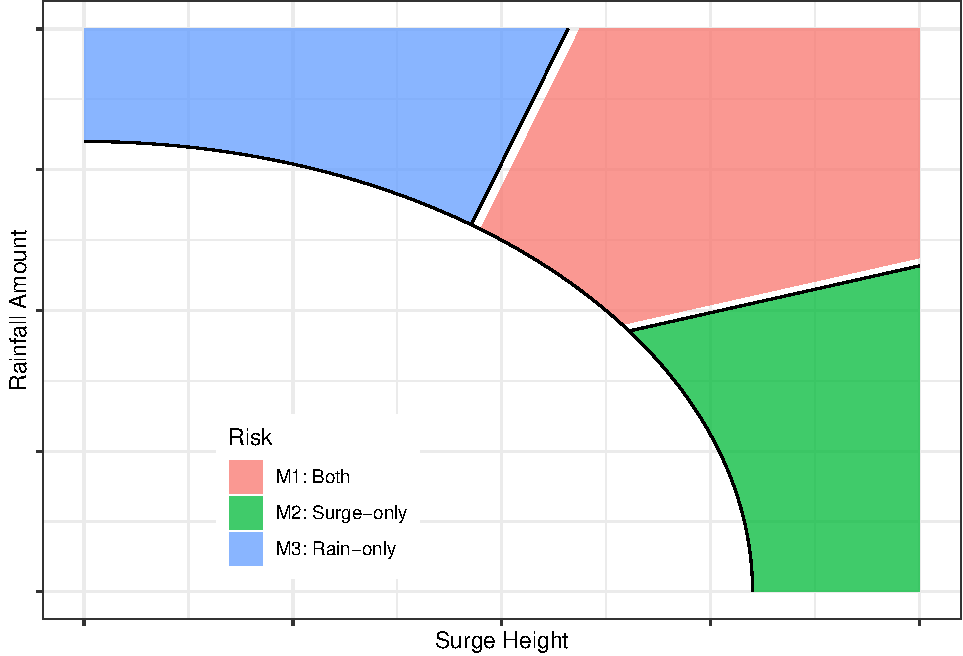
\includegraphics{draft_files/figure-latex/region a-1.pdf}

\begin{itemize}
\item
  Event based statistics
\item
  Aggregate rainfall
\item
  Period a sluice gate is open
\item
  Why we need to consider temporal trajectories and dependence in the
  plume
\end{itemize}

\section{Case Study}\label{case-study}

\begin{itemize}
\item
  Lake Lauwersoog (two sluices)
\item
  Show a plot of culmulative rainfall / surge / tide
\item
  How the sluice works (- 10)
\item
  Mechanisms in the Netherlands
\item
  Extremes don't necessary mean big - Duration is important
\item
  Largest != Longest
\item
  Define a surge period (clustering)
\item
  Importance of scoring the whole / understand trajectory
\end{itemize}

\section{Data}\label{data}

\begin{itemize}
\item
  Rainfall
\item
  Storm Surge
\item
  We treat tide (deterministic) and surge (random)
\item
  Caveat of wind (ignoring at present)
\item
  Seasonality
\end{itemize}

\section{Statistical Post-processing
Methods}\label{statistical-post-processing-methods}

\subsubsection{Univariate Methods}\label{univariate-methods}

\begin{itemize}
\tightlist
\item
  NGR
\end{itemize}

\subsubsection{Univariate Scoring}\label{univariate-scoring}

\begin{itemize}
\item
  Rank Histograms
\item
  CRPS
\item
  BSS
\end{itemize}

\subsection{Multivariate Methods}\label{multivariate-methods}

\begin{itemize}
\item
  ECC
\item
  Schaake (Analogs)
\end{itemize}

\subsection{Multivariate Scoring}\label{multivariate-scoring}

\begin{itemize}
\item
  ES
\item
  Variogram
\item
  Weights
\item
  David-Sebastiani (Not here)
\end{itemize}

\section{Results}\label{results}

\subsection{Surge Univariate}\label{surge-univariate}

\begin{itemize}
\item
  CRPS
\item
  BSS
\item
  Rank Histograms
\item
  Reliability (optional)
\end{itemize}

\subsection{Rainfall Univariate}\label{rainfall-univariate}

\begin{itemize}
\item
  CRPS
\item
  BSS
\item
  Rank Histograms
\item
  Reliability (optional)
\end{itemize}

\subsection{Surge Trajectory}\label{surge-trajectory}

\begin{itemize}
\item
  ES
\item
  VS
\item
  weights
\item
  relaximing to climatology (loose univariate skill)
\item
  best methods for restoring dependence
\end{itemize}

\subsection{Rainfall Trajectory}\label{rainfall-trajectory}

\begin{itemize}
\item
  ES
\item
  VS
\item
  weights
\item
  relaximing to climatology (loose univariate skill)
\item
  best methods for restoring dependence
\end{itemize}

\subsection{Combined Surge and Rainfall
Trajectories}\label{combined-surge-and-rainfall-trajectories}

\section{Discussion}\label{discussion}

\section{Conclusions}\label{conclusions}

\section{Future Directions}\label{future-directions}

\begin{itemize}
\item
  Wind
\item
  Bivariate post-processing (then restore dependence)
\item
  Lag relations (zheng/westra - explore)
\end{itemize}

\hypertarget{refs}{}
\hypertarget{ref-wahl_increasing_2015}{}
Wahl, Thomas, Shaleen Jain, Jens Bender, Steven D. Meyers, and Mark E.
Luther. 2015. ``Increasing Risk of Compound Flooding from Storm Surge
and Rainfall for Major US Cities.'' \emph{Nature Climate Change} 5 (12):
1093--7.
doi:\href{https://doi.org/10.1038/nclimate2736}{10.1038/nclimate2736}.

\hypertarget{ref-zheng_modeling_2014}{}
Zheng, Feifei, Seth Westra, Michael Leonard, and Scott A. Sisson. 2014.
``Modeling Dependence Between Extreme Rainfall and Storm Surge to
Estimate Coastal Flooding Risk.'' \emph{Water Resources Research} 50
(3): 2050--71.
doi:\href{https://doi.org/10.1002/2013WR014616}{10.1002/2013WR014616}.

\hypertarget{ref-zscheischler_dependence_2017}{}
Zscheischler, Jakob, and Sonia I. Seneviratne. 2017. ``Dependence of
Drivers Affects Risks Associated with Compound Events.'' \emph{Science
Advances} 3 (6): e1700263.
doi:\href{https://doi.org/10.1126/sciadv.1700263}{10.1126/sciadv.1700263}.

\end{document}
